\section{The distinguishing power of degree-aware MPNNs}\label{sec:dMPNNs}
We next turn our attention to degree-aware MPNNs, i.e., MPNNs whose message functions depend on the previous labels \textit{and} the degrees of the vertices involved.
Quintessential examples of degree-aware MPNNs (or dMPNNs for short) are the graph convolutional networks, introduced by~\cite{kipf-loose}. These networks are of the form
$$
\mathbf{L}^{(t)}:=\sigma\Bigl(\bigl(\mathbf{D}+\mathbf{I}\bigr)^{-1/2} (\mathbf{A}+\mathbf{I})\bigl(\mathbf{D}+\mathbf{I}\bigr)^{-1/2} \mathbf{L}^{(t-1)}\mathbf{W}^{(t)}\Bigr),
$$
as already described and phrased a dMPNN in Example~\ref{ex:KipfasMPNN}. In fact, many commonly used graph neural networks use degree information. We list a couple of such networks in Table~\ref{tab:dMPNNs}. It is easily verified that these can all be cast as dMPNNs along the same lines as Example~\ref{ex:KipfasMPNN}.

\begin{table}[]
\hrule
\hspace*{1ex}
 \caption{Various graph neural network formalisms which correspond to degree-aware MPNNs. All formalisms can be extended with a bias matrix $\mathbf{B}^{(t)}$ consisting of copies of the same row $\mathbf{b}^{(t)}$.}
    \label{tab:dMPNNs}
    \centering
    \begin{tabular}{ll}
 $\mathbf{L}^{(t)}:=\sigma\left(\mathbf{D}^{-1}\mathbf{A}\mathbf{L}^{(t-1)}\mathbf{W}^{(t)}\right)$ &\cite{} \\
$
\mathbf{L}^{(t)}:=\sigma\left(\mathbf{D}^{-1/2}\mathbf{A}\mathbf{D}^{-1/2}\mathbf{L}^{(t-1)}\mathbf{W}^{(t)}\right)$&\cite{} \\
$
\mathbf{L}^{(t)}:=\sigma\left((\mathbf{D}+\mathbf{I})^{-1}(\mathbf{A}+\mathbf{I})\mathbf{L}^{(t-1)}\mathbf{W}^{(t)}\right)$&\cite{} \\
$\mathbf{L}^{(t)}:=\sigma\left(\mathbf{L}^{(t-1)}\mathbf{W}_1^{(t)}+\mathbf{D}^{-1/2}\mathbf{A}\mathbf{D}^{-1/2}\mathbf{L}^{(t-1)}\mathbf{W}_2^{(t)}\right)$&\cite{} \\
$
\mathbf{L}^{(t)}:=\sigma\left((\mathbf{D}^{-1/2}\mathbf{A}\mathbf{D}^{-1/2}+\mathbf{I})\mathbf{L}^{(t-1)}\mathbf{W}^{(t)}\right)$ &\cite{} \\
$
\mathbf{L}^{(t)}:=\sigma\Bigl(\bigl(\mathbf{D}+\mathbf{I}\bigr)^{-1/2} (\mathbf{A}+p\mathbf{I})\bigl(\mathbf{D}+\mathbf{I}\bigr)^{-1/2} \mathbf{L}^{(t-1)}\mathbf{W}^{(t)}\Bigr)
$& \cite{kipf-loose} \\
$\mathbf{L}^{(t)}:=\sigma\left((r\mathbf{I}+(1-r)\tilde{\mathbf{D}})^{-1/2}(\mathbf{A}+p\mathbf{I})(r\mathbf{I}+(1-r)\mathbf{D})^{-1/2}\mathbf{L}^{(t-1)}\mathbf{W}^{(t)}\right)$ & \cite{DBLP:journals/corr/abs-1905-03046} 
    \end{tabular}
\hspace*{1ex}
\hrule
\end{table}
We denote by $\architecture_{\textsl{deg}}$ the class of degree-aware MPNNs. Our first observation is that
$\architecture_{\textsl{deg}}$ are not weaker than $\architectureWL$. This somewhat contradicts claims made about, e.g., the GCNs by~\cite{kipf-loose}, in the literature.
\begin{proposition}
The class $\architecture_{\textsl{deg}}$ is not weaker than $\architectureWL$. As a consequence,  $\architecture_{\textsl{deg}}$ and  $\architectureano$ are not equally strong.
\end{proposition}
\begin{proof}
It suffices to provide a dMPNN $M$ and labelled graph $\langle G,\pmb{\nu}\rangle$ such that there exists a $t\geq 0$ such that $\pmb{\ell}_{M_{\textsl{WL}}}^{(t)}\not\sqsubseteq \pmb{\ell}_M^{(t)}$. We construct an $M$ originating
from a GCN~\cite{kipf-loose}.
Consider the labelled graph $\langle G,\pmb{\nu})$ (\raisebox{-2ex}{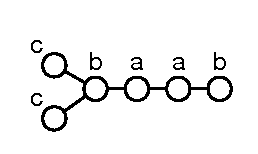
\includegraphics[height=1cm]{graph1}}) with 
vertex labelling  $\pmb{\nu}_{v_1}=\pmb{\nu}_{v_2}=[1,0,0]$,
$\pmb{\nu}_{v_3}=\pmb{\nu}_{v_6}=[0,1,0]$ and $\pmb{\nu}_{v_4}=\pmb{\nu}_{v_5}=[0,0,1]$. 
% The corresponding adjacency and degree matrices are given by:
% $$
% \mathbf{A}=\begin{bmatrix}
% 0 & 0 & 1 & 0 & 0 & 0\\
% 0 & 0 & 1 & 0 & 0 & 0\\
% 1 & 1 & 0 & 1 & 0 & 0\\
% 0 & 0 & 1 & 0 & 1 & 0\\
% 0 & 0 & 0 & 1 & 0 & 1\\
% 0 & 0 & 0 & 0 & 1 & 0
% \end{bmatrix}\text{ and } 
% \mathbf{D}=
% \begin{bmatrix}
% 1 & 0 & 0 & 0 & 0 & 0\\
% 0 & 1 & 0 & 0 & 0 & 0\\
% 0 & 0 & 3 & 0 & 0 & 0\\
% 0 & 0 & 0 & 2 & 0 & 0\\
% 0 & 0 & 0 & 0 & 2 & 0\\
% 0 & 0 & 0 & 0 & 0 & 1
% \end{bmatrix}.
% $$
We define $M$ such that for round $t=1$ and $\mathbf{x},\mathbf{y}\in\mathbb{A}^3$:
\begin{align*}
\textsc{Msg}^{(1)}\left(\mathbf{x},\mathbf{y},v,u\right)&:=
\frac{1}{d_v}\left(\frac{1}{1+d_v}\right)\mathbf{x}\left[\begin{smallmatrix}
1 & 0 & 0\\
0 & 1 & 0\\
0 & 0 & 1
\end{smallmatrix}\right]+
\left(\frac{1}{\sqrt{1+d_v}}\right)\left(\frac{1}{\sqrt{1+d_u}}\right)\mathbf{y}\left[\begin{smallmatrix}
1 & 0 & 0\\
0 & 1 & 0\\
0 & 0 & 1
\end{smallmatrix}\right]
\intertext{and} \textsc{Upd}^{(1)}(\mathbf{x},\mathbf{y})&:=\text{ReLU}(\mathbf{y}).
\end{align*}
% We consider $\mathbf{F}^{(1)}:=\sigma(\tilde{\mathbf{D}}^{-1/2}(\mathbf{A}+\mathbf{I})\tilde{\mathbf{D}}^{-1/2}\mathbf{F}^{(0)}\mathbf{W}^{(0)})$ with  $
% \mathbf{F}^{(0)}=
% \left[\begin{smallmatrix}
% 1 & 0 & 0\\
% 1 & 0 & 0\\
% 0 & 1 & 0\\
% 0 & 0 & 1\\
% 0 & 0 & 1\\
% 0 & 1 & 0\\
% \end{smallmatrix}\right]
% $ and choose $\mathbf{W}^{(0)}=\left[\begin{smallmatrix}
% 1 & 0 & 0\\
% 0 & 1 & 0\\
% 0 & 0 & 1
% \end{smallmatrix}\right]$. 
% We remark that $\pmb{\ell}^{(0)}:=\pmb{\ell}\equiv \mathbf{F}^{(0)}$.
It can be verified that 
$$
\pmb{\ell}_M^{(1)}=\begin{bmatrix}
\frac{1}{2} & \frac{1}{2\sqrt{2}}& 0\\
\frac{1}{2} & \frac{1}{2\sqrt{2}}& 0\\
\frac{1}{2\sqrt{2}} & \frac{1}{4}& \frac{1}{
2\sqrt{3}}\\
0 & \frac{1}{2\sqrt{3}}& \frac{2}{
3}\\
0 & \frac{1}{\sqrt{6}}& \frac{2}{
3}\\
0 & \frac{1}{2}& \frac{1}{
\sqrt{6}}
\end{bmatrix}.
$$
We observe that 
$(\pmb{\ell}_M^{(1)})_{v_4}\neq (\pmb{\ell}_M^{(1)})_{v_5}$. 
We note, however, that $$
(\pmb{\ell}_{M_\textsl{WL}}^{(1)})_{v_4}=\textsc{Hash}((0,0,1),\ldbl(0,0,1),(0,1,0\rdbl)=(\pmb{\ell}_{M_\textsl{WL}}^{(1)})_{v_5}.$$
Hence, 
$\pmb{\ell}_{M_{\textsl{WL}}}^{(1)}\not\sqsubseteq \pmb{\ell}_M^{(1)}$.
% $\pmb{\ell}^{(1)}\not\sqsubseteq \mathbf{F}^{(1)}$ and this architecture is not bounded by WL, without the additional constant factor $1$.
% In accordance with Proposition~\ref{prop:boundnonconstantR}, one can verify
% that $\pmb{\ell}^{(2)}\sqsubseteq \mathbf{F}^{(1)}$.
%  % We know, however, that it is bounded by WL on $(G,\pmb{\ell}{}^{(1)})$.
% \qed
% % It can, however, be verified that $\pmb{\ell}^{(2)}\sqsubseteq \mathbf{F}^{(1)}$.
% % \todo{The latter inclusion needs to be verified}\qed

The claim that $\architecture_{\textsl{deg}}$ and  $\architectureano$ are not equally strong, now follows easily. Indeed, if they were equally expressive
then by Proposition~\ref{prop:equalstrong}, $\architecture_{\textsl{deg}}$ would be equally strong as
$\architectureWL$. This contradicts with what we have shown above. Of course, $\architectureano$ is weaker than $\architecture_{\textsl{deg}}$, simply because any aMPNN is a dMPNN.
\end{proof}


% \begin{enumerate}
% %  \item \emph{Neighbourhood only.} When $\bW_1^{(t)}$ is always the $0$ matrix. The examples we consider are
% %  \begin{description}
% % % \item[\textit{Adjacency}:]
% % % % $\mathbf{L}=\mathbf{R}:=\mathbf{I}$, $p=q:=0$. Hence,
% % % $
% % % \mathbf{F}^{(t+1)}:=\sigma\left(\mathbf{A}\mathbf{F}^{(t)}\mathbf{W}^{(t)}\right)
% % % $
% % \item[\textit{Random walk (RW-GNN)}:] 
% % % $\mathbf{L}:=\mathbf{D}^{-1}$ with $\mathbf{D}$ the degree matrix of $\mathbf{A}$, $\mathbf{R}:=\mathbf{I}$, $p=q:=0$. Hence,
% % $$
% % \mathbf{F}^{(t)}:=\sigma\left(\mathbf{D}^{-1}\mathbf{A}\mathbf{F}^{(t-1)}\mathbf{W}^{(t-1)}\right);$$
% % \item[\textit{Augmented random walk (RW-GNN+)}:] 
% % % $\mathbf{L}:=\tilde{\mathbf{D}}^{-1}$ with $\tilde{\mathbf{D}}$ the degree matrix of $\mathbf{A}+\mathbf{I}$, $\mathbf{R}:=\mathbf{I}$, $p:=1$, $q:=0$. Hence,
% % $$
% % \mathbf{F}^{(t)}:=\sigma\left(\tilde{\mathbf{D}}^{-1}(\mathbf{A}+\mathbf{I})\mathbf{F}^{(t-1)}\mathbf{W}^{(t-1)}\right),$$
% % with $\tilde{\mathbf{D}}$ the degree matrix of $\mathbf{A}+\mathbf{I}$;
% % \item[\textit{Normalized adjacency (NA-GNN)}:] 
% % % $\mathbf{L}=\mathbf{R}:=\mathbf{D}^{-1/2}$, $p=q:=0$. Hence,
% % $$
% % \mathbf{F}^{(t)}:=\sigma\left(\mathbf{D}^{-1/2}\mathbf{A}\mathbf{D}^{-1/2}\mathbf{F}^{(t-1)}\mathbf{W}^{(t-1)}\right)
% % ;$$
% % \end{description}
% % \item \emph{Degree normalised.} Without restrictions on $\bW_1^{(t)}$ but fixing $\bN = \mathbf{D}^{-1/2}\mathbf{A}\mathbf{D}^{-1/2}$. For example
% % \begin{description}
% % \item[\textit{$1$st Order GCN (1-GCN)}:]
% % $$
% % \mathbf{F}^{(t)}:=\sigma\left(\mathbf{F}^{(t-1)}\mathbf{W}_1^{(t-1)}+\mathbf{D}^{-1/2}\mathbf{A}\mathbf{D}^{-1/2}\mathbf{F}^{(t-1)}\mathbf{W}_2^{(t-1)}\right);$$

% % \item[\textit{Simplified $1$st Order GCN (1-GCNs)}:]
% % $$
% % \mathbf{F}^{(t)}:=\sigma\left((\mathbf{D}^{-1/2}\mathbf{A}\mathbf{D}^{-1/2}+\mathbf{I})\mathbf{F}^{(t-1)}\mathbf{W}_2^{(t-1)}\right);$$
% % \end{description}

% % \item \emph{Normalised and optimised.} These are the remaining architectures.
% % \begin{description}
% % \item[\textit{Augmented adjacency (NA-GNN+)}~\cite{kipf-loose}:] % $\mathbf{L}=\mathbf{R}:=\tilde{\mathbf{D}}^{-1/2}$, $p:=1$, $q:=0$. Hence,
% % $$
% % \mathbf{F}^{(t)}:=\sigma\left(\tilde{\mathbf{D}}^{-1/2}(\mathbf{A}+\mathbf{I})\tilde{\mathbf{D}}^{-1/2}\mathbf{F}^{(t-1)}\mathbf{W}^{(t-1)}\right);
% % $$
% \item[\textit{Weighted augmented adjacency (NA-GNN++)}~\cite{DBLP:journals/corr/abs-1905-03046}:]
% $$\mathbf{F}^{(t)}:=\sigma\left((r\mathbf{I}+(1-r)\tilde{\mathbf{D}})^{-1/2}(\mathbf{A}+p\mathbf{I})(r\mathbf{I}+(1-r)\mathbf{D})^{-1/2}\mathbf{F}^{(t-1)}\mathbf{W}^{(t-1)}\right),
% $$
% which underlies the PiNet architecture.
% \end{description}
% \end{enumerate}



% One of the example graph neural architectures that was cast as an MPNN by \citet{GilmerSRVD17}
% was the GCN architecture by~\citet{KipfW16}. In that architecture~\footnote{We note that we here identify the vertex labeling $\pmb{\ell}^{(t)}$ with its vector in $\mathbb{A}^s$.}, for each round $t=1,2,\ldots,d$,
% \begin{equation}
% \pmb{\ell}^{(t)}:=\sigma\Bigl(\bigl(\mathbf{D}+\mathbf{I}\bigr)^{-1/2} (\mathbf{A}+\mathbf{I})\bigl(\mathbf{D}+\mathbf{I}\bigr)^{-1/2} \pmb{\ell}^{(t-1)}\mathbf{W}\Bigr), \label{GNN:Kipf}
% \end{equation}
% where $\mathbf{A}$ denotes the adjacency matrix of the input graph, $\mathbf{D}$ is the diagonal matrix holding the degree of the vertices on its diagonal, and $\mathbf{I}$ is the identity matrix. Finally, $\sigma$ is a non-linear activation function such as sign or ReLU. To capture this architecture we  introduce \textit{degree-aware} MPNNs, of dMPNNs for short. These are MPNNs
% whose message functions $\textsc{Msg}^{(t)}$ depend on the intermediate features $\pmb{\ell}^{(t-1)}_v$ and $\pmb{\ell}^{(t-1)}_w$, and furthermore on $d_v$ and $d_w$. They are not allowed to depend on  $v$ and $w$.

% It is readily observed that we can see architectures of the form~(\ref{GNN:Kipf}) as a dMPNNs by defining for each $(w,v)\in E^*$
% \begin{align*}
% \mathbf{m}_{v\gets w}^{(t)}&:=	
% \textsc{Msg}(\pmb{\ell}^{(t-1)}_v,\pmb{\ell}^{(t-1)}_w,d_v,d_w)=
% 	\left(\frac{1}{\sqrt{1+d_v}}\right)	\left(\frac{1}{\sqrt{1+d_w}}\right)((\pmb{\ell}^{(t-1)}_w)^{\textsc{t}}\mathbf{W})^{\textsc{t}}\\
% \pmb{\ell}_v^{(t)}&:=\textsc{Upd}\left(\sum_{w\in N_G^*(v)} \mathbf{m}_{v\gets w}^{(t)}\right)=
% \sigma\left(\sum_{w\in N_G^*(v)} \mathbf{m}_{v\gets w}^{(t)})\right).
% \end{align*}

The previous proposition begs the question how anonymous MPNNs and degree-aware MPNNs are related. To answer this question we observe that anonymous MPNNs can compute the degrees of vertices in one round of computation.

\begin{lemma}
	The degrees of all vertices can be obtained in one round of computation of an anonymous MPNN. Furthermore, this degree information can be encoded together with the initial labelling $\pmb{\nu}$ of $G$.
	\end{lemma}
\begin{proof}
We can assume, without loss of generality, that the labelled graph $\langle G,\pmb{\nu}\rangle$ is such that
$\pmb{\nu}:V\to\mathbb{A}^{s+1}$ and where the last entry in every label is equal to $0$.
We then define the aMPNN
$M_d$ with the following message and update functions.
For each $\mathbf{x}=(\mathbf{x}',x)$ and $\mathbf{y}=(\mathbf{y}',y)$ in $\mathbb{A}^{s+1}$, vertices $v$ and $u\in N_G(v)$, and each $t\geq 1$:
$$
\textsc{Msg}^{(t)}(\mathbf{x},\mathbf{y},v,w):=(\mathbf{x}',1)
\text{ and } \textsc{Upd}^{(t)}(\mathbf{x},\mathbf{y}):=
\begin{cases}
\mathbf{x} & y=0\\
(\frac{1}{y}\mathbf{y}',y) & y\neq 0
\end{cases}.
$$
Then,
$
\mathbf{m}_v^{(1)}:=\sum_{u\in N_G(v)}(\mathbf{x}',1)=(d_v\mathbf{x}',d_v)
$ and $\textsc{Upd}^{(1)}_v=(\mathbf{x}',d_v)$.
In other words, after round $1$, each vertex knows its own degree, represented in its label. This implies that
$(\pmb{\ell}_M^{(1)})_v=(\pmb{\mu}_v,d_v)$, as desired.
% Then, for round $t=1$, we first define for each $(w,v)\in E^*$, 
% $$\mathbf{m}^{(1)}_{v\gets w}=\textsc{Msg}(\pmb{\ell}^{(0)}_v,\pmb{\ell}^{(0)}_{w},\pmb{\eta}_{(w,v)}):=\left[\begin{smallmatrix}1\\\pmb{\nu}\end{smallmatrix}\right]\in\mathbf{Q}^{s+1}.$$ Then, for any
% $\left[\begin{smallmatrix} a\\\mathbf{b}\end{smallmatrix}\right]\in \mathbb{A}^{s+1}$ with $a\neq 0$, we 
% let 
% $$\textsc{Upd}\left(\begin{bmatrix} a\\\mathbf{b}\end{bmatrix}\right):=\begin{bmatrix} a\\\frac{1}{a}\mathbf{b}\end{bmatrix}.
% $$
% It is now clear that $\textsc{Upd}\left(\sum_{w\in N_G^*(v)}\mathbf{m}_{v\gets w}^{(t)}\right)=\left[\begin{smallmatrix} d_v\\\pmb{\nu}\end{smallmatrix}\right]\in \mathbb{A}^{s+1}$.
\end{proof}

The following proposition now follows almost immediately.
\begin{proposition}\label{prop:onestep}
The class $\architecture_{\textsl{deg}}$ is weaker than 
$\architectureano$, with $1$ step ahead.
\end{proposition}
\begin{proof}
As in the previous lemma we assume that the labelling
$\pmb{\nu}$ of $G$ is such that $\pmb{\nu}:V\to\mathbb{A}^{s+1}$ with its last entries equal to $0$. Take an arbitrary 
\end{proof}

% As an immediate corollary of Propositions~\ref{prop:WL} and~\ref{prop:onestep},  we obtain:
% \begin{corollary}
% 	The distinguish power of dMPNNs is bounded by WL, with a factor of one.
% \end{corollary}

% As a consequence, we cannot rely on Proposition~\ref{prop:WL} to  upper bound
% the distinguishing power of graph neural networks whose propagation rules rely on the degrees
% (such the GCNs by ~\citep{KipfW16}). In the literature, however, it is often mentioned that
% GCNs by ~\citep{KipfW16} are bounded by WL, hereby referring to \citep{XuHLJ19,grohewl}.
% This is, strictly speaking, not correct.
%
% To provide a correct upper bound, we  We denote dMPNNs the class of degree-aware MPNNs.
% In the next section, we study dMPNNs in more detail.

% \section{The distinguishing power of dMPNNs}
%
%
%
% We show that dMPNNs are still bounded by WL, but are in general on step ahead. This may explain the success of such architectures for graph related classification tasks.
%
% \begin{proposition}
% 	Degree-aware MPNNs are bounded by WL, with a factor of one.
% \end{proposition}
%
% As check, let us model the GCNs by \citep{KipfW16} as dMPNNs. We recall from \citet{KipfW16}
% that features are obtained as:
% $$\mathbf{F}^{(t)}:=\sigma(\tilde{D}{}^{-1/2}\tilde{\mathbf{A}}\tilde{\mathbf{D}}{}^{-1}\mathbf{F}^{(t-1)}\mathbf{W}).$$
% It is readily observed that we can see this as a dMPNNs by defining for each $(w,v)\in E^*$
% \begin{align*}
% \mathbf{m}_v^{(t)}&:=
% \textsc{Msg}(\mathbf{F}_{v\bullet}^{(t-1)},\mathbf{F}_{v\bullet}^{(t-1)},d_v,d_w)=
% 	\left(\frac{1}{\sqrt{1+d_v}}\right)	\left(\frac{1}{\sqrt{1+d_w}}\right)\mathbf{F}_{w\bullet}^{(t-1)}\mathbf{W}\\
% \mathbf{F}_v^{(t)}&:=\textsc{Upd}(\sum_{w\in N_G^*(v)} \mathbf{m}_w^{(t)})=
% \sigma\left(\sum_{w\in N_G^*(v)} \mathbf{m}_w^{(t)})\right).
% \end{align*}

\begin{corollary}
	The GCNs by \citet{KipfW16} are bounded by WL, but with a factor of one.
\end{corollary}
This corollary more correctly states the relationship between these GCNs and WL.




\smallskip
\noindent
\leftpointright
One possible additional insight is that dMPNNS can be defined such that
the message functions  only depend on $d_w$ and the features. That is, we 
can eliminate the dependency on $d_v$.
Indeed, to see this, one just adds one extra entry with value $1$ to $\mathbf{m}_v^{(t)}$ by adjusting the definition of $\textsc{Msg}$. Then, when summing over
$w\in N_G^*(v)$, these values add up to $d_v$, and $\textsc{Upd}$ can be defined such that it takes $d_v$ into account when aggregating the features. 
As a consequence, when GNN architectures use degree information, but only use $d_v$, then the dMPPNs is in fact an aMPNN and the WL bound holds. This basically corresponds to our current understanding between the asymmetry of $\mathbf{L}$ and $\mathbf{R}$. 







% We have seen two restricted classes of MPNNs in the previous section: Anonymous MPNNs and degree-aware MPNNs. Together, these classes suffice to capture many common graph neural network architectures. In this section we study their distinguishing power. The take-away message from this section is that degree-aware MPNNs (such as those originating from the GCN architecture by~\cite{kipf-loose}, see Example~\ref{ex:KipfasMPNN}) have a slightly stronger distinguishing power than anonymous MPNNs. This may explain the experimental success of graph neural networks such as the GCNs by~\cite{kipf-loose}. Despite being based on a simple observation, the difference between anonymous and degree-aware MPNNs has, to our knowledge, not been reported in the literature before. In fact, one often finds statements indicating that existing results for anonymous MPNNs \cite{xhlj19,grohewl} carry over verbatim for, say the GCN architecture
% by~\cite{kipf-loose}. As we will see, this is not precisely true.
% \looseness=-1

% This section is organised as follows. We first define how two classes of MPNNs can be compared relative to  their distinguishing power (Section~\ref{subsec:compare}). We then recall known results for anonymous MPNNs (Section~\ref{subsec:aMPNNs}). We conclude by establishing the distinguishing power of degree-aware MPNNs (Section~\ref{subsec:dMPNNs}).



% % These notions can be generalised to classes of MPNNs, just as we did in Definition~\ref{def:classesweak}. 
% % \begin{definition}\normalfont
% % Consider two classes $\architecture_1$ and $\architecture_2$ of MPNNs.
% % Then, $\architecture_1$ is said to be weaker than $\architecture_2$, but may be $c$ steps ahead, if for every $M_1\in \architecture_1$
% % there exists an $M_2\in\architecture_2$ such that $M_1$ is weaker than $M_2$, but may be $c$ steps ahead. Similarly,
% %  $\architecture_1$ is said to be weaker than $\architecture_2$, possibly up to a linear factor $c'$ and $c$ steps ahead, if for every $M_1\in \architecture_1$
% % there exists an $M_2\in\architecture_2$ such that $M_1$ is weaker than $M_2$, possibly up to a linear factor $c'$ and  $c$ steps ahead. 
% % \qed
% % \end{definition}

% % 
% % The following observation follows immediately from the definitions. Consider two classes $\architecture_1$ and $\architecture_2$ of MPNNs. Let $c$ and $c'$ be arbitrary
% % constants.
% % If $\architecture_1$ is weaker than $\architecture_2$, then $\architecture_1$ is weaker than $\architecture_2$, but may be $c$ steps ahead. If $\architecture_1$ is weaker than $\architecture_2$, but may be $c$ steps ahead, then $\architecture_1$ is weaker than $\architecture_2$, possibly up to a linear factor $c'$  and $c$ steps ahead. We will see that the reverse implication do not necessarily hold later in the paper.

% % We finally observe that when 

% % The following definition states when one class of MPNNs is weaker (in terms of distinguishing power) than another class of MPNNs. Intuitively, one class $\architecture$ will be weaker than other class $\architecture'$ if any MPNN $M\in\architecture$ cannot distinguish more vertices than some MPNN $M'\in\architecture'$.

% % \begin{definition}\label{def:comparing}\normalfont
% % Consider two classes $\architecture$ and $\architecture'$ of MPNNs. We say that $\architecture$ is weaker than $\architecture'$ (or equivalently that $\architecture'$ is stronger than $\architecture$) if there exists a function $g:\mathbb{N}\to \mathbb{N}$ such that for every $M \in \architecture$ there exists an $M'\in \architecture'$ satisfying $\pmb{\ell}_{M'}^{(g(t))}\sqsubseteq \pmb{\ell}_{M}^{(t)}$, for all $t\geq 0$ and for any labeled graph $( G,\pmb{\nu},\pmb{\eta})$. This is denoted by $\architecture \sqsubseteq \architecture'$.
% % % with $d$ layers 
% % % and every labelling $\labl$ compatible with $g$ there exists $g' \in \architecture'$ with $m'$ layers such that $g'(\labl) \sqsubseteq g(\labl)$.
% % % This is denoted by $\architecture' \sqsubseteq \architecture$.
% % We write $\architecture \not \sqsubseteq \architecture'$ if the above property does not hold. 
% % If we additionally require that the function $g:\mathbb{N}\to\mathbb{N}$ satisfies 
% % $g(t)\le t +c$ for some constant $c$, then we write that $\architecture \sqsubseteq \architecture'$ up to a constant factor $c$. In the particular case when this holds for $c = 0$ we write that $\architecture \sqsubseteq \architecture'$ with no factor. Similarly, if there exist constants $c, c'$ such that $g(t) \le ct + c'$ we write that $\architecture \sqsubseteq \architecture'$ up to a linear factor $c$.
% % \end{definition}




% % Of particular interest will be the class of MPNNs corresponding to the WL algorithm. 
% % \floris{Ok, add aMPNN description of WL. Note that I added the description of the WL algorithm on undirected graphs but with each labels to the prelims. }
% % We will denote this class by $\architectureWL$ and it is defined as MPNNs in which the message 
% % We say that an architecture $\architecture$ is \emph{bounded by WL} if $\architecture\sqsubseteq \architectureWL$. We also say that an architecture $\architecture$ is \emph{WL-strong} if $\architectureWL \sqsubseteq \architecture$. The definitions of bounded by WL and WL-strong up to linear and constant factors carry on in the obvious way.

% \subsection{Anonymous MPNNs}\label{subsec:aMPNNs}


% % Following the work by~\cite{xhlj19} and~\cite{grohewl}, which relates to anonymous MPNNs, we study the distinguishing power of degree-aware MPNNs. We will see that degree-aware MPNNs (such as those originating from the GCN architecture by~\cite{kipf-loose}, see Example~\ref{ex:KipfasMPNN}) have a slightly stronger distinguishing power than anonymous MPNNs.
% % More precisely, any labeling computed by $d$ rounds of a degree-aware MPNNs can be computed by $d+1$ rounds of an anonymous MPNN. This may explain the experimental success of graph neural networks such as the GCNs by~\cite{kipf-loose}. We note that in the literature one often does not distinguish between anonymous and degree-aware MPNNs
% % and 
% % Before showing this, we first define how two classes of MPNNs can be compared relative to
